\documentclass[12pt,a4paper]{article}
\usepackage[a4paper,left=3cm,right=3cm,top=2.5cm,bottom=2.5cm]{geometry}
\usepackage{fontspec}
\setmainfont{Times New Roman}
\usepackage{graphicx}

\newcommand{\noindentfix}{\vspace{10pt}\noindent}
\newcommand{\chapterheader}[1]{{\noindent\fontsize{18}{14}\textbf{#1}\vspace{2pt}}}
\newcommand{\subchapterheader}[1]{{\noindent\fontsize{16}{14}\textbf{#1}\vspace{2pt}}}

\usepackage{polyglossia}
\setdefaultlanguage{slovak}
\setotherlanguage{english}

\begin{document}

    % TODO: Title page

    \chapterheader{Rozbor riešenia}

    \noindentfix Môj regulárny výraz bol výraz \texttt{[a]b\{a|b\}}:
    \begin{figure}[h]
        \centering
        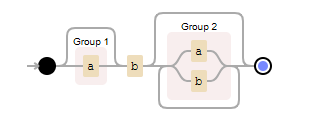
\includegraphics{./stavovy-diagram-pre-regularny-vyraz.png}
        \caption{Stavový diagram pre regulárny výraz \texttt{(a)?b(a|b)*}.}
        \label{fig:stavovy-diagram}
    \end{figure}

    \noindentfix Teda, na prvej pozícii sa vyskytuje 0 alebo 1 znakov \textbf{a}, nasleduje jeden znak \textbf{b} a potom sa vyskytuje 0 alebo viac znakov \textbf{a} alebo \textbf{b}.

    \noindentfix Akceptovanými reťazcami môže byť napríklad:
    \begin{itemize}
        \setlength{\parskip}{0pt}
        \setlength{\itemsep}{0pt}
        \item \texttt{ab}
        \item \texttt{abba}
        \item \texttt{b}
        \item \texttt{bba}
    \end{itemize}

    \noindentfix Naopak neakceptovanými reťazcami môžu byť:
    \begin{itemize}
        \setlength{\parskip}{0pt}
        \setlength{\itemsep}{0pt}
        \item \texttt{a}
        \item \texttt{aabb}
        \item \texttt{aa}
        \item \texttt{aab}
    \end{itemize}

    \noindentfix Pri riešení zadania som sa rozhodol pre programovací jazyk Java a využiť nástroj Maven pre testovanie výrazov.

    \noindentfix Ako prvá vec, ktorú som urobil, bolo vytvorenie nového Maven projektu. Najprv som vytvoril konfiguračný súbor \texttt{pom.xml}, do ktorého som nastavil základné parametre pre projekt (názov, verziu Javy a pod.) a následne inicializoval vytvorený projekt príkazom \texttt{mvn clean install}.

    \pagebreak
    \subchapterheader{Algoritmus}

    \noindentfix Zo zadania som vyčítal, že nemôžem použiť knižnice pre regulárne výrazy. Pre riešenie je možné využiť buď jeden cyklus \texttt{while}, počas ktorého budem odoberať zo vstupného reťazca znaky podľa stavu, alebo využiť rekurzívne funkcie a tým elimininovať potrebu cyklu. V riešení som sa rozhodol pre využitie cyklu \texttt{while}.

    \noindentfix V cykle budem odoberať znaky podľa stavov dovtedy, dokým mi neostane prázdny reťazec, alebo nevyskytne chyba. Chybou je nesplnenie jednej z požiadaviek cyklu (výstupom programu je znak "N"). Ak sa nevyskytne chyba a program prejde celým reťazcom bez problémov, potom výstupom je znak "A".

    \noindentfix Pre zjednodušenie kódu som presunul kontrolu stavu $q_1$ do osobitnej metódy.

    % TODO: Referencie?

\end{document}